
\section{Wirtschaftliche Ausarbeitung}
\subsection{Marktforschung}
\begin{frame}
\frametitle{Marktforschung}
\begin{itemize}
\item Ziel: Ausschlaggebende Eigenschaften einer Registrierkassensoftware feststellen (für Konkurrenzanalyse)
\item wurde mittels Fragebögen durchgeführt
\item 1.Fragebogen: Wichtige Eigenschaften einer Registrierkassensaftware feststellen
\item 2.Fragebogen: Diese Eigenschaften nach ihrer Wichtigkeit anordnen
\end{itemize}
\end{frame}
\begin{frame}
\frametitle{Marktforschung}
Ergebnis
\begin{itemize}
\item Funktionalität: 13 Punkte
\item Laufsicherheit: 15 Punkte
\item Preis: 17 Punkte
\item Bedienbarkeit/Benutzerfreundlichkeit: 17 Punkte
\item Hardwareunabhängigkeit: 21 Punkte
\item Übersichtlichkeit: 22 Punkte
\item andere: 35 Punkte
\end{itemize}
\end{frame}
\subsection{Konkurrenzanalyse}
\begin{frame}
\frametitle{Konkurrenzanalyse}
\begin{itemize}
\item Ziel: Determinieren ob ein Eintritt in den Markt sinnvoll wäre, Festellen ob der Markt weiter unterteilt werden kann
\item Konkurrenten wurden anhand ihrer Relevanz priorisiert (Google)
\item Methodik des Stärken-Schwächen-Profils wurde verwendet
\end{itemize}
\end{frame}
\begin{frame}
\frametitle{Konkurrenzanalyse}
\begin{figure}
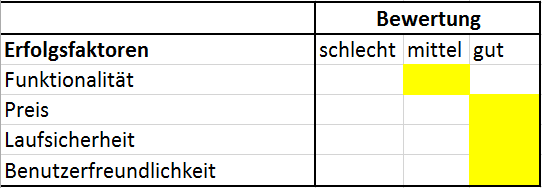
\includegraphics[scale=0.6]{Idealprofil}
\caption{Idealprofil}
\end{figure}
\end{frame}
\begin{frame}
\frametitle{Konkurrenzanalyse}
Ergebnis:
\newline
\begin{itemize}
\item Eintritt in den Markt ist nicht sinnvoll
\item Der Markt kann nicht weiter segmentiert werden
\end{itemize}
\end{frame}
\subsection{Break-Even-Point-Analyse}
\begin{frame}
\frametitle{Break-Even-Point-Analyse}
\begin{itemize}
\item Ziel: Determinieren wann sich der Absatz dieser Registrierkassensoftware rentieren würde
\item Kosten: Entwicklungskosten, Serverbetriebskosten
\item Break-Even-Point: Alle Kosten gedeckt und Einkommen gegeben
\end{itemize}
\end{frame}
\begin{frame}
\frametitle{Break-Even-Point-Analyse}
\begin{figure}
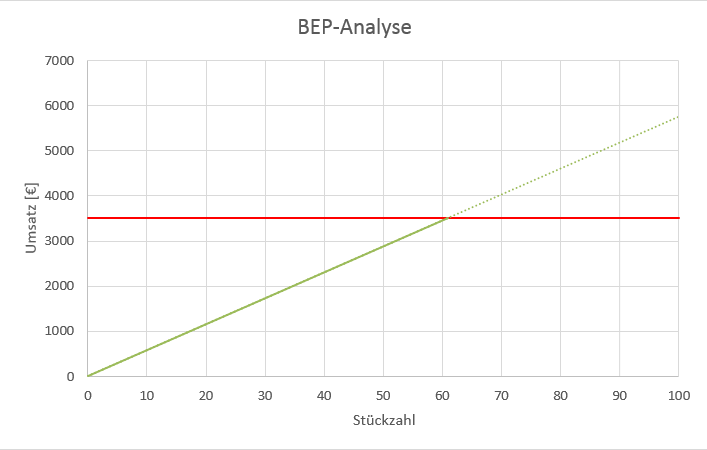
\includegraphics[scale=0.45]{BEP}
\end{figure}
\end{frame}

